\documentclass[
  12pt,
  openright,
  twoside,
  a4paper,
  english,
  brazil
]{abntex2}

\usepackage{indentfirst}
\usepackage{pdfpages}
\usepackage[alf]{abntex2cite}
\usepackage{booktabs}
\usepackage{pifont}

\titulo{Implementação de um front end para IR LLVM}
\tituloestrangeiro{Implementing a LLVM IR front end}

\autor{Bernardo Ferrari Mendonça}
\local{Brasil}
\data{2019}
\orientador{Rafael de Santiago}
\coorientador{Evandro}
\instituicao{
  Universidade Federal de Santa Catarina
  \par
  Departamento de Informática e Estatística
  \par
  Ciência da Computação
}

\tipotrabalho{Trabalho de Conclusão de Curso de Graduação}

\preambulo{Proposta de monografia submetida ao Programa
de Graduação em Ciência da Computação
para a obtenção do Grau de Bacharel.}

\begin{document}
\pretextual{}
\imprimircapa{}
\imprimirfolhaderosto{}

\begin{folhadeaprovacao}
  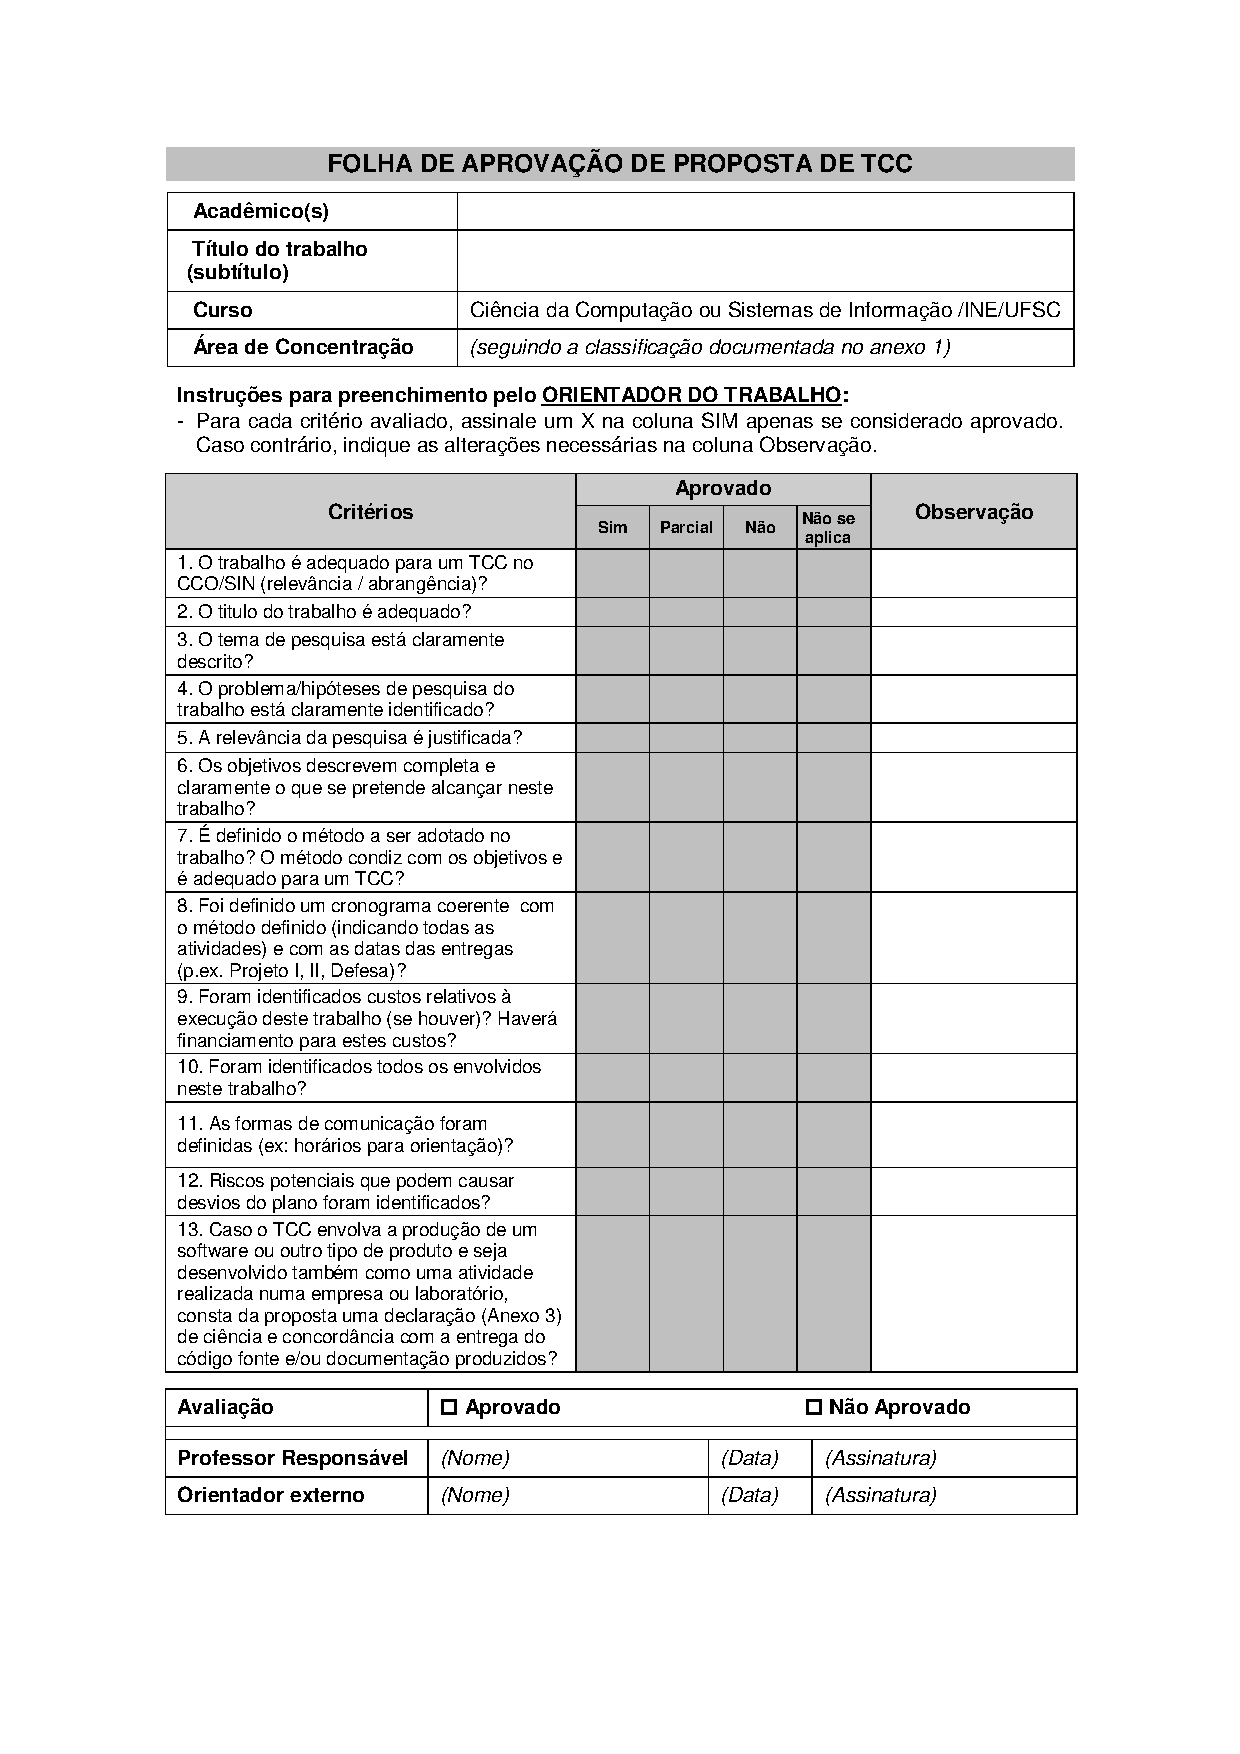
\includepdf{folha-de-aprovacao.pdf}
\end{folhadeaprovacao}

\begin{resumo}
Meu resumo.

\vspace{\onelineskip}
\noindent
\textbf{Palavras-chave}: minhas\@. palavras\@. chave.

\end{resumo}

\begin{KeepFromToc}
  \tableofcontents
\end{KeepFromToc}

\textual{}

\chapter{Introdução}\label{cap:introdução}

Esta vai ser minha introdução\cite{dijkstra1968}!

\chapter{Objetivos}\label{cap:objetivos}

O principal objetivo deste trabalho consiste em projetar, implementar e avaliar uma linguagem de programação similar a linguagem de programação c.
Esta implementação de linguagem de programação deve fazer uso do ecossistema llvm, incluindo suas ferramentas para geração de linguagem de representação intermediaria, para otimização de código e para geração de código objeto executável.

\section{Objetivos específicos}

Os objetivos específicos são:
\begin{itemize}
  \item Projetar uma linguagem de programação similar a c;
  \item Implementar um analisador léxico, um analisador sintático e uma tradução dirigida a sintaxe;
  \item Fazer um estudo sobre a linguagem intermediaria llvm;
  \item Implementar uma ferramenta para controlar a otimização da linguagem intermediaria llvm. Além de controlar a tradução da mesma para código objeto;
  \item Fazer um estudo sobre o processo de ligação de código;
  \item Integrar a ferramenta ao processo de ligação de código do ambiente GNU/Linux;
  \item Avaliar as decisões de projeto da linguagem de programação projetada quanto a linguagem c.
\end{itemize}

\chapter{Método de pesquisa}\label{cap:metodo_de_pesquisa}

\chapter{Cronograma}\label{cap:cronograma}

O cronograma é descrito pela tabela~\ref{tab:cronograma} abaixo.

\begin{table}[h!]
  \caption{Planejamento das etapas do trabalho de conclusão de curso}\label{tab:cronograma}
  \resizebox{\textwidth}{!}{
    \begin{tabular}{@{}lcccccccccccccc@{}}
      \toprule
      \multicolumn{1}{c}{Etapas} & \multicolumn{13}{c}{Messes} \\
      \cmidrule(lr){2-15}
      & \multicolumn{2}{c}{2019} & \multicolumn{12}{c}{2020} \\
      \cmidrule(lr){2-3} \cmidrule(lr){4-15}
      & nov & dez & jan & fev & mar & abr & mai & jun & jul & ago & set & out & nov & dez \\
      \midrule
      Entrega da proposta completa
      &04/11&&&&&&&&&&&&&\\
      Estudo da fundamentação teórica
      &\ding{55}&\ding{55}&\ding{55}&\ding{55}&\ding{55}&\ding{55}&&&&&&&&\\
      Desenvolvimento da solução
      &&&\ding{55}&\ding{55}&\ding{55}&\ding{55}&\ding{55}&\ding{55}&\ding{55}&\ding{55}&&&\\
      Desenvolvimento do relatório de Projeto I
      &&&&&&\ding{55}&\ding{55}&\ding{55}&&&&&\\
      Entrega do relatório de Projeto I
      &&&&&&&&\ding{55}&&&&&\\
      Redação do rascunho do TCC
      &&&&&&&&&\ding{55}&\ding{55}&&&&\\
      Desenvolvimento do rascunho do TCC
      &&&&&&&&&&\ding{55}&\ding{55}&\ding{55}&&\\
      Entrega do rascunho do TCC
      &&&&&&&&&&&&\ding{55}&&\\
      Preparação da defesa pública
      &&&&&&&&&&&&\ding{55}&\ding{55}&\\
      Defesa pública
      &&&&&&&&&&&&&\ding{55}&\\
      Ajustes no relatório final do TCC
      &&&&&&&&&&&&&\ding{55}&\ding{55}\\
      \bottomrule
    \end{tabular}
  }
\end{table}

\chapter{Custos}\label{cap:custos}

Não há custos envolvidos.

\chapter{Recursos humanos}\label{cap:recursos_humanos}

\chapter{Comunicação}\label{cap:comunicacao}

\chapter{Riscos}\label{cap:riscos}

\postextual{}

\bibliography{bibliography.bib}

\end{document}
